\documentclass{article}
\usepackage[utf8]{inputenc}
\usepackage{fullpage}
\usepackage{amsmath}
\usepackage{amsfonts}
\usepackage{amssymb}
\usepackage{subfiles}
\usepackage{blindtext}
\usepackage{xspace}
\usepackage[dvipsnames]{xcolor}
\usepackage{tikz}
\usetikzlibrary{automata, positioning, arrows}

\setcounter{MaxMatrixCols}{10}

\newtheorem{theorem}{Theorem}
\newtheorem{remark}[theorem]{Remark}

%--- mCRL2 ---%
\font \aap cmmi10
\newcommand{\at}[1]{\mbox{\aap ,} #1}
\newcommand{\ap}{{:}}
\newcommand{\tuple}[1]{\ensuremath{\langle {#1} \rangle}}
\newcommand{\vars}{\mathit{vars}}
\newcommand{\up}{\blacktriangle}
\newcommand{\down}{\blacktriangledown}
\newcommand{\concat}{\ensuremath{+\!\!+\:}}
\newcommand{\aftertime}{\ensuremath{<\!\!<}}
\newcommand{\emptymap}{\ensuremath{\{ : \}}}
\newcommand{\emptylist}{\ensuremath{[\:]}}
\newcommand{\stochasticstate}[2]{\ensuremath{\{#1 \mapsto #2\}}}

%--- automata ---%
\tikzset{
  ->, >=stealth', shorten >=1pt, semithick,
  auto, node distance=6em,
  every state/.style={very thick},
  initial text=$ $
}

\title{Confluence Detection}
\author{Wieger Wesselink}
\date{September 2019}

\begin{document}

\maketitle

\section{Confluence}
Consider the following untimed linear process specification $P$, with initial state $d_0$.

\[
\begin{array}{l}
P(d)=
\sum\limits_{i\in I}\sum\limits_{e_i}c_i(d, e_i)\rightarrow a_i(f_i(d,e_i)) \cdot P(g_i(d,e_i))
\end{array}
\]
We distinguish different kinds of confluence. Let summand $j \in I$ be the index of a $\tau$-summand, and $i \in I$ be the index of an arbitrary summand.
In the sequel we abbreviate $c_i(d,e_i)$ $f_i(d,e_i)$ and $g_i(d,e_i)$ with $c_i$, $f_i$ and $g_i$. Note that for the $\tau$-summand with index $j$ we have $a_j = \tau$ and $f_j = []$.

\subsection{Trivial confluence}

Trivial confluence is defined as

\begin{equation*}
\begin{array}{l}
C_{trivial}(i, j) = \forall d, e_i, e_j : (c_i \land c_j) \Rightarrow  
      (a_i = \tau) 
     \land (g_i = g_j)
\end{array}
\end{equation*}
Note that trivial confluence only applies to $\tau$-summands. In isolation it is not a very useful property to check.

\subsection{Triangular confluence}

Triangular confluence is defined as

\begin{equation*}
\begin{array}{l}
C_{triangular}(i, j) = \forall d, e_i, e_j : (c_i \land c_j) \Rightarrow
      (c_i[d := g_j]
\land (f_i = f_i[d := g_j])
\land (g_i[d := g_j] = g_i))
\end{array}
\end{equation*}

\subsection{Commutative confluence}

Commutative confluence is defined as

\begin{equation}
\begin{array}{l}
C_{commutative}(i, j) = C_{trivial}(i, j) \lor \forall d, e_i, e_j : (c_i \land c_j) \Rightarrow
\quad \exists e'_i, e'_j  : \\
\qquad \begin{array}{ll}
(& \\
      & c_i[d := g_j, e_i := e'_i)] \\
\quad \land & c_j[d := g_i, e_j := e'_j] \\
\quad \land & (f_i = f_i[d := g_j, e_i := e'_i]) \\
\quad \land & (g_i[d := g_j, e_i := e'_i] = g_j[d := g_i, e_j := e'_j])\\
)&
\end{array} \\
\end{array}
\end{equation}
The reason for adding the term $C_{trivial}(i, j)$ is probably that otherwise a simple $\tau$-summand like 
\[ (n=0) \rightarrow \tau \cdot P(n=1) \]
is not even confluent with itself. 

\subsection{Square confluence}

Square confluence is defined as

\begin{equation*}
\begin{array}{l}
C_{square}(i, j) = C_{trivial}(i, j) \lor \forall d, e_i, e_j : (c_i \land c_j) \Rightarrow 
      c_i[d := g_j]
\land c_j[d := g_i]
\land (f_i = f_i[d := g_j]) 
\land (g_i[d := g_j] = g_j[d := g_i]))
\end{array}
\end{equation*}
It is obtained from $C_{commutative}(i,j)$ by taking $e'_i = e_i$ and $e'_j = e_j$.

\newpage

\begin{figure}
\begin{center}
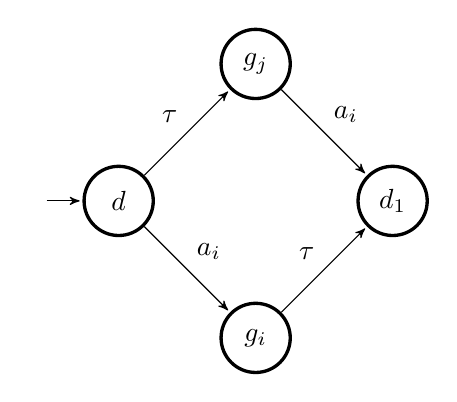
\begin{tikzpicture}[node distance=7em, , scale=1.0, transform shape]
    % States
    \node[state,initial]   (d)                      {$d$};
    \node[state]           (gj)  [above right of=d] {$g_j$};
    \node[state]           (gi)  [below right of=d] {$g_i$};
    \node[state]           (d1)  [below right of=gj] {$d_1$};
    % Transitions
    \path[->]
      (d)  edge node {$\tau$} (gj)
      (d)  edge node {$a_i$}  (gi)
      (gi) edge node {$\tau$}  (d1)
      (gj) edge node {$a_i$} (d1);
\end{tikzpicture}
\end{center}
\caption{square commutative confluence, with $d_1 = g_j[d:=g_i]$}
\end{figure}

\begin{figure}
\begin{center}
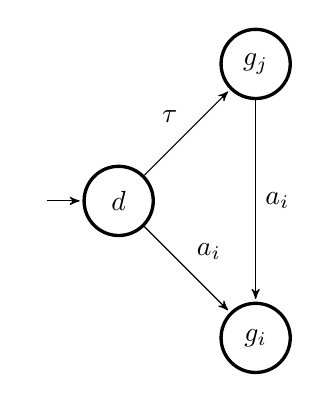
\begin{tikzpicture}[node distance=7em, , scale=1.0, transform shape]
    % States
    \node[state,initial]   (d)                      {$d$};
    \node[state]           (gj)  [above right of=d] {$g_j$};
    \node[state]           (gi)  [below right of=d] {$g_i$};
    % Transitions
    \path[->]
      (d)  edge node {$\tau$} (gj)
      (d)  edge node {$a_i$}  (gi)
      (gj) edge node {$a_i$}  (gi);
\end{tikzpicture}
\end{center}
\caption{triangular confluence}
\end{figure}

\begin{figure}
\begin{center}
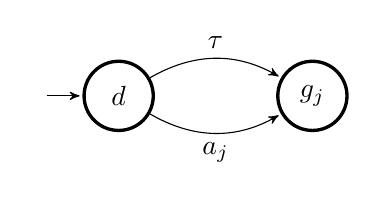
\begin{tikzpicture}[node distance=7em, , scale=1.0, transform shape]
    % States
    \node[state,initial]   (d)                {$d$};
    \node[state]           (gj)  [right of=d] {$g_j$};
    % Transitions
    \path[->]
      (d)  edge[bend left, above] node {$\tau$} (gj)
      (d)  edge[bend right, below] node {$a_j$} (gj);
\end{tikzpicture}
\end{center}
\caption{trivial confluence, with $a_j = \tau$}
\end{figure}

\end{document}

